%~~~~~~~~~~~~~~~~~~~~~~~~~~~~~~~~~~~~~~~~~~~~~~~~~~~~~~~~~~~~~~~~~~~~~~~
\section{Filtro de Bloom}\label{sec:bloom}
%~~~~~~~~~~~~~~~~~~~~~~~~~~~~~~~~~~~~~~~~~~~~~~~~~~~~~~~~~~~~~~~~~~~~~~~

Um filtro de Bloom é uma estrutura de dados probabilística que representa um conjunto e permite verificar a pertinência de elementos com tolerância a falsos positivos \cite{bloom1970space}. É uma representação bastante compacta: são necessários menos de 10 bits por elemento para uma probabilidade 1\% de falsos positivos \cite{bonomi2006improved}. 

Nas Seções \ref{sec:bloom:def} e \ref{sec:bloom:example}, apresentamos a definição da estrutura Filtro de Bloom e mostramos um exemplo compreensivo de seu funcionamento. Na Seção~\ref{sec:bloom:false}, calculamos a probabilidade de falsos positivos inerentes ao algoritmo. Na Seção~\ref{sec:bloom:cardinality}, introduzimos uma técnica para estimar cardinalidade de conjuntos utilizando filtro de Bloom. Na Seção~\ref{sec:bloom:counting}, discutimos em detalhe umas das variantes importantes da estrutura que permite remoção de elementos. Outras variantes são discutidas na Seção~\ref{sec:bloom:variants}. Na Seção~\ref{sec:bloom:apps} apresentamos algumas aplicações de filtros de Bloom. E na Seção~\ref{sec:bloom:experiments} mostramos o resultado de experimentos com filtros de Bloom, que visam avaliar o erro observado em uma implementação real.

\subsection{Definição}\label{sec:bloom:def}

Um filtro de Bloom representa um conjunto $S$ de cardinalidade $n$ utilizando um vetor $B$ de $m$ bits. Inicialmente, $B[i] = 0\ \forall\ i \in [1..m]$. O filtro está associado a $k$ funções \emph{hash} $h_i : S \rightarrow [1..m]\ \forall\ i \in [1..k]$. Assume-se que cada função $h_i$ mapeia elementos de $S$ para o intervalo $[1..m]$ de forma aleatória com uma distribuição uniforme.

Para inserir um elemento, é preciso atribuir 1 para cada posição no filtro mapeada pelas funções $h_i$, como mostra o Algoritmo~\ref{alg:bloominsert}.

\begin{algorithm}
\linespread{1}\selectfont
\caption{Adiciona um elemento a um filtro de Bloom}
\label{alg:bloominsert}
\begin{algorithmic}[1]
\Procedure{Inserir}{$x$}
    \For{$i \gets  1 \textrm{ to } k$}
        \State $B[h_i(x)] \gets 1$
	\EndFor
\EndProcedure
\end{algorithmic}
\end{algorithm}

Analogamente, para verificar se um elemento pertence a um conjunto, é preciso verificar se todos os bits mapeados pelas funções $h_i$ estão ligados, i.e., um elemento $x$ provavelmente pertence ao conjunto $S$ se o Algoritmo~\ref{alg:bloomquery} retorna verdadeiro.

\begin{algorithm}
\linespread{1}\selectfont
\caption{Verifica se um elemento pertence a um filtro de Bloom}
\label{alg:bloomquery}
\begin{algorithmic}[1]
\Function{Verificar}{$x$}
    \State $resultado \gets \textbf{true}$ 
    \For{$i \gets  1 \textrm{ to } k$}
        \State $resultado \gets resultado \land B[h_i(x)] = 1$
	\EndFor
	\Return $resultado$
\EndFunction
\end{algorithmic}
\end{algorithm}

A Figura~\ref{fig:bloom1} mostra um exemplo de filtro de Bloom. Do lado esquerdo, estão representadas as operações de inserção, utilizando duas funções \emph{hash}. Do lado direito, as operações de verificação. Importante notar que a última operação de verificação trata o caso de um falso posivito, pois o elemento não existe de fato no conjunto previamente inserido.

\begin{figure}[!htbp]
  \centering
  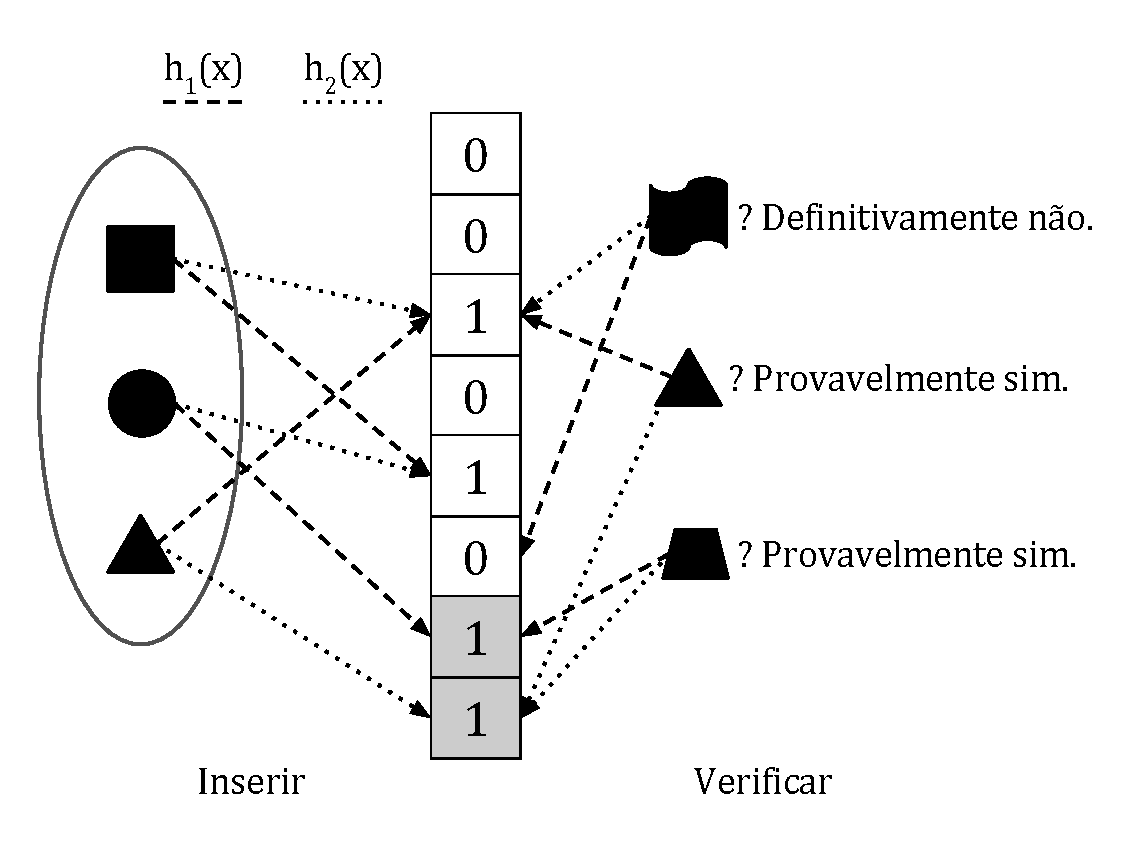
\includegraphics[scale=0.45]{files/bloom1.pdf}
  \caption{Exemplo de filtro de bloom}
  \label{fig:bloom1}
\end{figure}

Em sua forma mais simples, o funcionamento de um filtro de Bloom é similar ao de uma \emph{hash table} tradicional, porém os elementos originais não são armazenados. Em vez disso, apenas um bit é usado para representar a pertinência do \emph{hash} do elemento na tabela. Além disso, múltiplas funções \emph{hash} são utilizadas.

Assim como em \emph{hash tables}, pode haver colisões nos filtros de Bloom. Portanto, falsos positivos são possíveis. Falsos negativos por sua vez não são possíveis Este comportamento é desejado em sistemas que precisam evitar operações custosas (por exemplo, acesso a disco, comunicação de rede, etc.) em casos onde não seja realmente necessário. 

Para diminuir a probabilidade de colisão, é preciso dimensionar o filtro e as funções \emph{hash} baseados no número de elementos esperados. Por exemplo, usando 7 funções e pouco menos de 10 bits por elemento no filtro, é possível garantir uma probabilidade de falsos positivos menor que 1\% \cite{bonomi2006improved}. É possível determinar a quantidade ótima de bits e funções dada uma probabilidade esperada de falsos positivos.

O número de funções \emph{hash} pode posar como um desafio, a princípio. Porém, é resultado conhecido que apenas duas funções independentes são suficientes para gerar qualquer número de funções sem perda das propriedades originais da estrutura \cite{kirsch2006less}.

Em termos de operações suportadas, filtros de Bloom permitem atualização incremental, bem como união entre filtros (que para filtros de mesmo número de bits, consiste em um \emph{OU binário} entre eles). Entretanto, em sua forma mais simples, não suportam remoção de elementos nem interseção entre filtros sem introduzir falsos negativos ou afetar as probabilidades de falsos positivos. Diversas variações e extensões aos filtros de Bloom foram propostas, algumas discutidas nas Seções \ref{sec:bloom:counting} e \ref{sec:bloom:variants}.

\subsection{Exemplo}\label{sec:bloom:example}


\subsection{Probabilidade de falso positivo}\label{sec:bloom:false}

A probabilidade de um falso positivo é determinada pela probabilidade de colisão. Assim, quanto mais bits forem usados no filtro de Bloom, menor a probabilidade de um falso positivo. Para diminuir a probabilidade de colisões é possível também utilizar múltiplas funções \emph{hash} para cada elemento, mas somente até um certo ponto, onde realizar múltiplos hashes por elemento acaba aumentando a probabilidade de colisões.

É possível calcular a probabilidade de um falso positivo. Considere uma tabela $B[1..m]$, após inserir $n$ elementos e usando $k$ funções \emph{hash}. Se $X_i$ é a variável aleatória que fornece o valor de $B[i]$, então:
\[
\Pr[X_i = 0] = \Pr\left[\bigwedge_{x \in X, 1 \leq j \leq k} h_j(x) \neq i \right] = \left( 1 - \frac{1}{m}\right)^{kn}
\]

Seja \textsc{FalsoPositivo} o evento do filtro reportar pertinência para um elemento $x \notin X$. Logo, a probabilidade de haver um falso positivo é a mesma de encontrar $k$ bits 1 aleatoriamente na tabela, ou seja:
\[
\Pr[\textsc{FalsoPositivo}] = \Pr\left[\bigwedge_{1 \leq j \leq k} X_{h_j(x)} = 1 \right] = \left( 1 - \left( 1 - \frac{1}{m}\right)^{kn} \right)^k \approx \left( 1 - \mathrm{e} ^{-kn/m} \right)^k
\]

É fácil ver que a probabilidade de falsos positivos cresce conforme $n$ cresce. Por isso, é preciso dimensionar o filtro de Bloom de acordo com o número de elementos no conjunto. Se definirmos $q = m/n$ (quantidade de bits por elemento, reescrevemos a última probabilidade como:
\[
\Pr[\textsc{FalsoPositivo}] \approx \left( 1 - \mathrm{e} ^{-k/q} \right)^k
\]

A Figura~\ref{fig:probfalso1} mostra como esta probabilidade se comporta para diferentes valores de $k$ e $q$.

\begin{figure}[!htbp]
\centering
\scalebox{0.80}{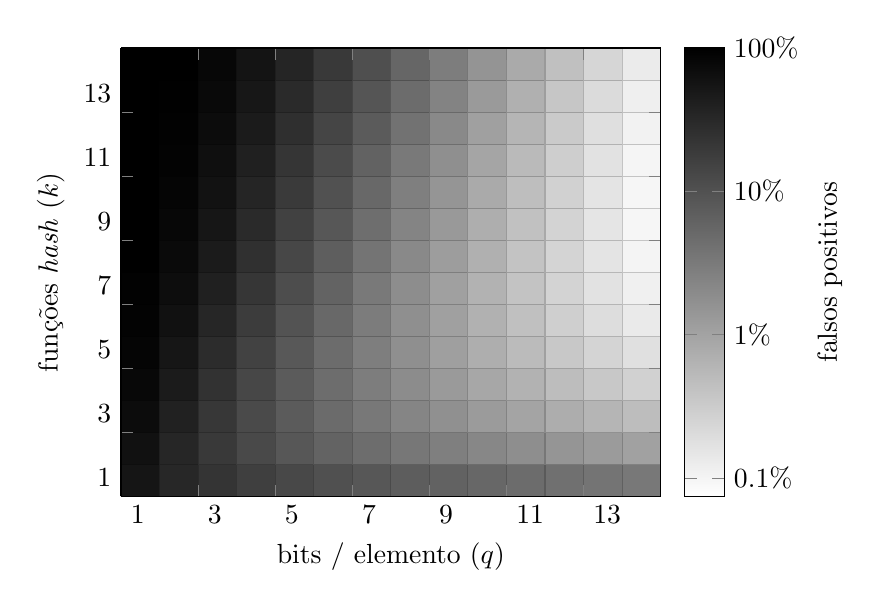
\begin{tikzpicture}[
        declare function = {
            p(\q,\k) = ((1 - (e^(-\k/\q)))^\k)*100;
        }
    ]
    \begin{axis}[
        view={0}{90}, 
        colorbar, 
        colorbar style={
            ylabel=falsos positivos,
            yticklabels={0, 0.1\%, 1\%, 10\%, 100\%},
        },
        colormap={}{ gray(0cm)=(1); gray(1cm)=(0);},
        xlabel=bits / elemento ($q$),
        ylabel=funções \emph{hash} ($k$),
        xticklabel style={anchor=north west},
        yticklabel style={anchor=south east},
        ytick = { 1, 3, ..., 14},
        xtick = { 1, 3, ..., 14},
        zmode=log,
        log base z=10,
    ]
        \addplot3[surf,domain=1:15,samples=15]{p(x,y)};
    \end{axis}
\end{tikzpicture}}
\caption{Probabilidade de falsos positivos}
\label{fig:probfalso1}
\end{figure}

Bonomi et al. \cite{bonomi2006improved} mostram ainda que a probabilidade é minimizada quando $k = q \ln 2$. Assim, é possível definir a probabilidade mínima de falsos positivos a partir do número de bits por elemento:
\[
\Pr[\textsc{FalsoPositivo}] = (1-e^{\ln(2)}) ^ {q \ln(2)} = ((1/2)^{\ln(2)})^q \approx \left( 0.6185 \right)^q
\]

É possível ver na Figura~\ref{fig:probfalso2} que a probabilidade de falsos positivos cai exponencialmente em relação ao número de bits por elemento no filtro.

\begin{figure}[!htbp]
\centering
\scalebox{0.80}{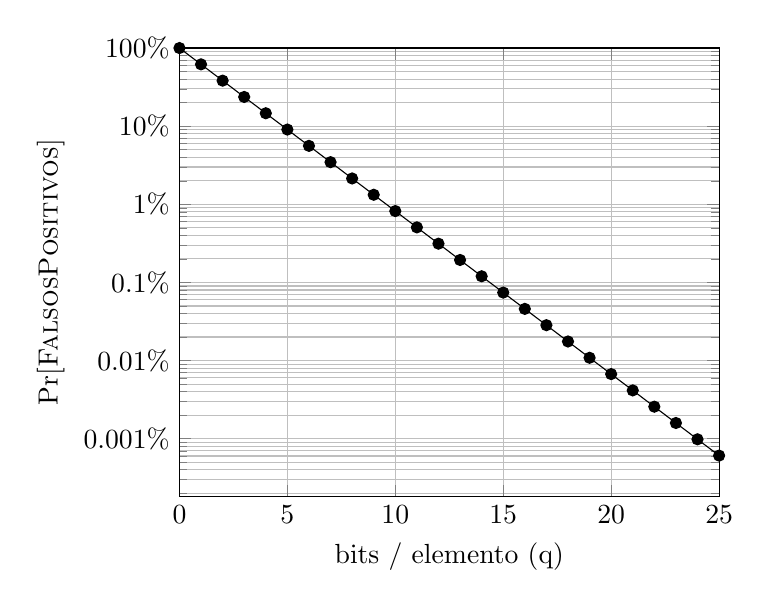
\begin{tikzpicture}[
        declare function = {
            p(\q) = (0.6185)^(\q);
        }
    ]
	\begin{axis}[
        grid=both,
        xlabel=bits / elemento (q),
		ylabel={Pr[\textsc{FalsosPositivos}]},
        yticklabels={0, 0.001\%, 0.01\%, 0.1\%, 1\%, 10\%, 100\%},
        ymode=log,
        ymax=1,
		xmin=0,
		xmax=25]
	\addplot[mark=*,domain=0:25,samples=26] {p(x)};
	\end{axis}
\end{tikzpicture}}
\caption{Probabilidade mínima de falsos positivos}
\label{fig:probfalso2}
\end{figure}

Desta forma, a escolha do número de bits por elemento torna-se crucial para dimensionar a quantidade de falsos positivos. Esta análise precisa ser feita \emph{a priori}, pois não é possível redimensionar um filtro de Bloom sem modificar suas propriedades estatísticas. 

Existem variações do algoritmo que mitigam este problema. Por exemplo, os \emph{Dynamic Bloom Filters} \cite{guo2010dynamic} colocam um limite superior na probabilidade de falso positivo criando um novo filtro quando o limite é ultrapassado, penalizando as consultas em um fator logaritmico, em relação ao tamnho do conjunto, pois precisam verificar vários filtros. 

Já os \emph{Block-partitioned Bloom Filters} \cite{papapetrou2010cardinality} penalizam tanto a inserção quanto a consulta de forma similar, porém por inserir e verificar os elementos em todos os filtros, mantêm as propriedades algébricas de união entre filtros através de operações booleanas entre seus vetores.

\subsection{Estimativa de cardinalidade}\label{sec:bloom:cardinality}

É possível estimar a cardinalidade do conjunto representado por um filtro de Bloom \cite{whang1990linear,papapetrou2010cardinality}. O princípio é análogo àquele empregado na Seção~\ref{sec:bloom:false} para estimar a probabilidade de falsos positivos. Seja $T$ a variável aleatória que representa o número de bits $1$ após inserir $n$ elementos num filtro $B[1..m]$ e $k$ funções \emph{hash}. Portanto, $T = \sum_{1 \leq i \leq m} X_i = 1$ e a esperança $E[T]$ é uma função $S(n)$ (para $m$ e $k$ fixos) tal que:
\[
E[T] = \sum_{1 \leq i \leq m} E[X_i] = m \times Pr[X_i = 1] = \hat{S}(n) = m \times \left( 1 - \left( 1 - \frac{1}{m}\right)^{kn} \right)
\]

Desta forma, é possível estimar $n$ a partir de $t$:
\[
\hat{n} = \hat{S}^{-1}(t) = \frac{\ln \left( 1 - \frac{t}{m} \right)}{k \times \ln \left( 1 - \frac{1}{m} \right)} \approx \frac{-m}{k} \times \ln \left( 1-\frac{t}{m} \right)
\]

Perceba que esta estimativa é extremamente dependente da quantidade de bits por elemento no filtro. Portanto, dado um certo filtro de Bloom, apenas um intervalo definido de cardinalidades tem um erro entro de um limite aceitável. Papapetrou et al. \cite{papapetrou2010cardinality} mostram que é possível definir um limite inferior na probabilidade da cardinalidade real estar num certo intervalo $(n_a, n_b)$ (com $\hat{S}^{-1}(t-1) \leq n_a \leq n_b \leq \hat{S}^{-1}(t+1)$). Esta probabilidade se dá pela fórmula:
\[
Pr[n_a \leq n \leq n_b] = 1 - e^{-\frac{(t+1-\hat{S}(n_b))^2}{2\hat{S}(n_b)}} - e^{t-1-\hat{S}(n_a)} \times \left( \hat{S}(n_a) / (t-1) \right)^{t-1}
\]

Este é apenas um limite inferior. Na prática é possível estimar valores bem maiores. Em especial, para estimar cardinalidades não há vantagens em utilizar múltiplas funções \emph{hash}, pois isto somente aumentaria a densidade de bits iguais a 1 no filtro. Whang et al. introduziram o algoritmo \textsc{Linear Counting} \cite{whang1990linear} que utiliza um filtro de Bloom com apenas uma função \emph{hash} para estimar a cardinalidade. Assim,
\[
\hat{n} \approx -m \times \ln \left( 1-\frac{t}{m} \right)
\]

Em  \cite{whang1990linear} também é mostrado que o erro padrão da estimativa está fortemente atrelada ao fator de carga, que consiste em quantos elementos distintos foram inseridos para cada bit na estrutura, ou $n/m$, expresso a seguir:
\[
\sigma_{\hat{n}} = \frac{\sqrt{m(e^{n/m} - (n/m) - 1)}}{n}
\]

Assim, assumindo um filtro com quantidades diversas de bits, é possível ver a degradação do erro padrão conforme o fator de carga aumenta (Figura \ref{fig:bloom_cardinality}).

\begin{figure}[!htbp]
\centering
\scalebox{0.80}{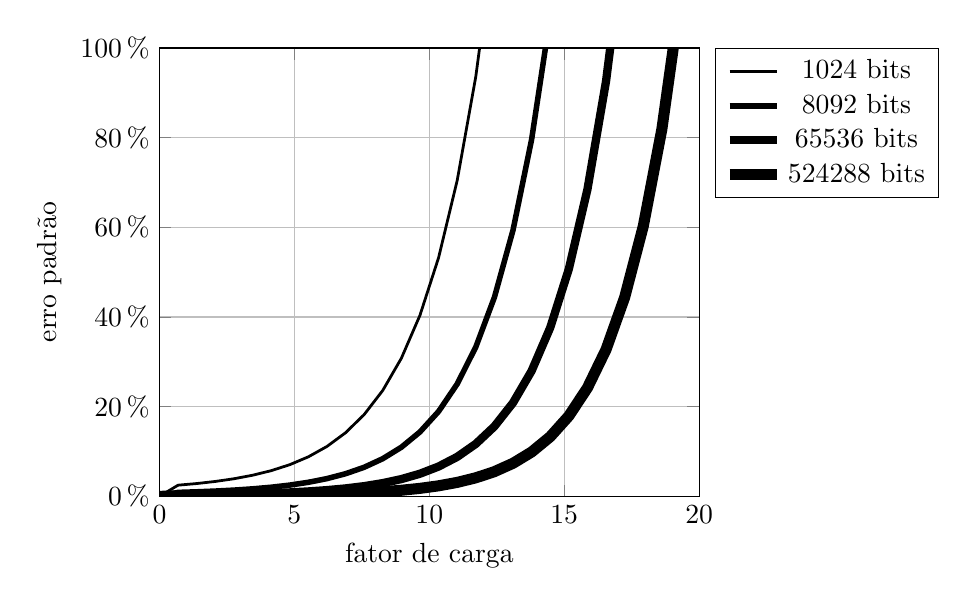
\begin{tikzpicture}[
        declare function = {
            p(\n,\m) = (\m*(e^(\n/\m) - (\n/\m) - 1)) ^ (1/2) / \n;
        }
    ]
	\begin{axis}[
	    scaled ticks=false, 
        grid=both,
        xlabel=fator de carga,
		ylabel=erro padrão,
		yticklabel=\pgfmathparse{100*\tick}\pgfmathprintnumber{\pgfmathresult}\,\%,
		ymin=0, ymax=1,
		xmin=0, xmax=20, 
		legend columns=1, 
	    legend style={legend pos=outer north east,}
    ]
    
    \addplot[line width=1pt,domain=0:20,samples=30]{p(1024*x, 1024)};
    \addplot[line width=2pt,domain=0:20,samples=30]{p(8092*x, 8092)};
    \addplot[line width=3pt,domain=0:20,samples=30]{p(65536*x, 65536)};
    \addplot[line width=4pt,domain=0:20,samples=30]{p(524288*x, 524288)};
	\legend{1024 bits, 8092 bits, 65536 bits, 524288 bits};

	\end{axis}
\end{tikzpicture}}
\caption{Erro padrão por fator de carga para filtros de vários tamanhos.}
\label{fig:bloom_cardinality}
\end{figure}


\subsection{\emph{Counting Bloom filters}}\label{sec:bloom:counting}

Em sua forma mais simples, o filtro de Bloom não permite remoção de elementos. Uma solução trivial para este problema, introduzida por Fan et al. \cite{fan1998summary}, é manter um contador de $b$ bits para cada posição no vetor $B$ do filtro.

Desta forma, as operações originais do filtro de Bloom são estendidas. A inserção passa a incrementar o valor de cada uma das posições resultantes das funções \emph{hash} (Algoritmo~\ref{alg:cbloominsert}). A remoção (Algoritmo~\ref{alg:cbloomremove}) e verificação (Algoritmo~\ref{alg:cbloomquery}) são análogas.


\begin{algorithm}[!htbp]
\linespread{1}\selectfont
\caption{Adiciona um elemento a um \emph{Counting Bloom Filter}}
\label{alg:cbloominsert}
\begin{algorithmic}[1]
\Procedure{Inserir}{$x$}
    \For{$i \gets  1 \textrm{ to } k$}
        \If{$B[h_i(x)] < 2^b-1$}
            \State $B[h_i(x)] \gets B[h_i(x)]+1$
        \EndIf
	\EndFor
\EndProcedure
\end{algorithmic}
\end{algorithm}

\begin{algorithm}[!htbp]
\linespread{1}\selectfont
\caption{Adiciona um elemento a um \emph{Counting Bloom Filter}}
\label{alg:cbloomremove}
\begin{algorithmic}[1]
\Procedure{Remover}{$x$}
    \For{$i \gets  1 \textrm{ to } k$}
        \If{$B[h_i(x)] < 2^b-1$}
            \State $B[h_i(x)] \gets B[h_i(x)]-1$
        \EndIf
	\EndFor
\EndProcedure
\end{algorithmic}
\end{algorithm}    

\begin{algorithm}[!htbp]
\linespread{1}\selectfont
\caption{Verifica se um elemento pertence a um \emph{Counting Bloom Filter}}
\label{alg:cbloomquery}
\begin{algorithmic}[1]
\Function{Verificar}{$x$}
    \State $resultado \gets \textbf{true}$ 
    \For{$i \gets 1 \textrm{ to } k$}
        \State $resultado \gets resultado \land B[h_i(x)] \geq 1$
	\EndFor
	\Return $resultado$
\EndFunction
\end{algorithmic}
\end{algorithm}

Agora a Figura~\ref{fig:bloom2} mostra um exemplo de filtro de Bloom com contagem. Do lado esquerdo figuram as operações de inserção, com duas funções \emph{hash}. Perceba que colisões incrementam a posição resultante no vetor. Do lado direito estão as verificações. Na terceira verificação nota-se um falso positivo.

\begin{figure}[!htbp]
  \centering
  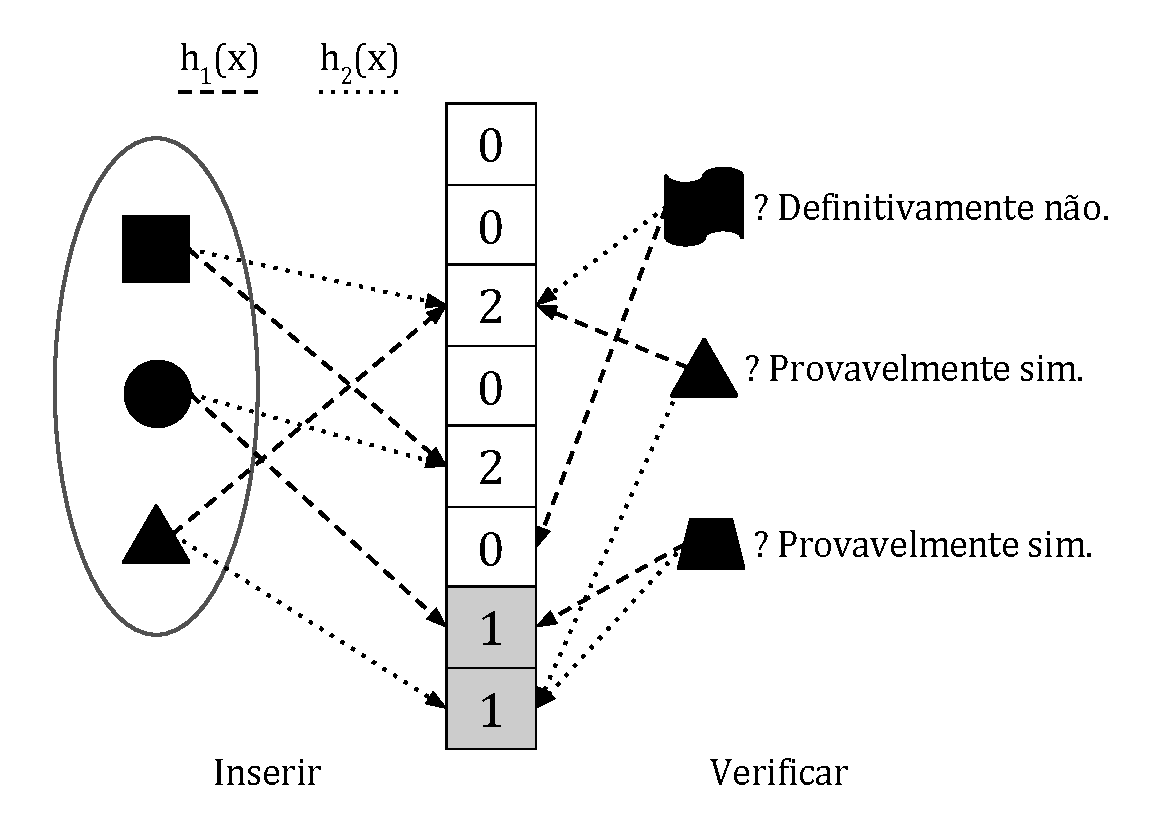
\includegraphics[scale=0.45]{files/bloom2.pdf}
  \caption{Exemplo de filtro de bloom com contagem}
  \label{fig:bloom2}
\end{figure}

A remoção neste filtro baseia-se na ausência de overflows em seus contadores. Para tanto, é preciso dimensionar o tamanho destes contadores de forma a minimizar a probabilidade de overflow. Como originalmente o filtro usa apenas um bit por posição no vetor, qualquer número de bits adicionais escolhidos para representar o contador aumenta significativamente o espaço necessário para armazenar a estrutura. Normalmente, 4 bits são suficientes para a maior parte das aplicações, o que faz com que estes filtros usem quatro vezes mais espaço que filtros normais.

O número de bits por contador determina a probabilidade de \emph{overflow}. \emph{Overflows} em \emph{counting Bloom filters} precisam ser ativamente tratados. Se um \emph{overflow} ocorrer é preciso manter o contador no máximo valor possível. De forma equivalente, ao tentar decrementar uma posição já no maior valor possível, é preciso mantê-la nesse mesmo valor. Faz-se isto para evitar a introdução de falsos negativos.

Na prática, entretanto, \emph{overflows} devem ser consideravelmente raros. A probabilidade de um \emph{overflow} dado que cada contador usa $b$ bits, após inserir $m$ elementos, usando 10 bits por elemento e otimizando o número de funções \emph{hash} é:
\[
Pr[\textsc{overflow}] \leq n \left( \frac{\mathrm{e} \ln 2}{2^b} \right)^{2^b}
\]
como provado por Fan et al. \cite{fan1998summary}. Assim, ao usar 4 bits para os contadores, a probabilidade de overflow concentra-se em:
\[
Pr[\textsc{overflow em 4 bits}] \leq 1.37 \times 10^{-15} \times n
\]

Esta probabilidade baseia-se na possibilidade de produzir funções \emph{hash} realmente aleatórias, o que pode ser aproximado, mas não pode ser garantido. Em um pior caso em especial, se o mesmo elemento for repetidamente oferecido à estrutura, a probabilidade de \emph{overflow} torna-se criticamente alta.

\subsection{Outras variantes}\label{sec:bloom:variants}

O filtro de Bloom, em sua simplicidade, tem limitações que posam como desafios para algumas aplicações. Desde sua concepção, entretanto, muitas extensões foram propostas para superar estas limitações (geralmente em detrimento de algum parâmetro de desempenho), entre elas:

\begin{description}

  \item[\emph{Compressed Bloom Filters} \cite{mitzenmacher2002compressed}] 
    Discute esquemas de compressão para otimizar o tamanho de filtros enviados através de rede ou salvos em disco. O objetivo é construir filtros com mais bits e menos funções \emph{hash}, de forma a minimizar o tamanho comprimido e/ou aumentar a precisão. Especialmente útil em caso de caches distribuídos. 

  \item[\emph{Distance-sensitive Bloom Filters} \cite{kirsch2006distance}] 
    Responde consultas do tipo "algum elemento próximo a $x$ pertence a $S$?", dada uma métrica apropriada, utilizando funções \emph{hash} sensíveis a localidade, com possibilidade tanto de falsos positivos como falsos negativos. Esta variante é bastante útil para detecção de plágio, por exemplo.

  \item[\emph{Dynamic Bloom Filters} \cite{guo2010dynamic}] 
    Permite redimensionar dinamicamente filtros de Bloom sem perder suas propriedades estatísticas. Baseia-se na criação de múltiplos filtros com um limite superior na probabilidade de falsos positivos, i.e., quando um filtro alcança uma taxa de falsos positivos muito alta, outro filtro vazio é criado. Nesta modalidade, a complexidade das operações padrão é maior, entretanto, na prática isso não posa como um problema. É possível dimensionar o tamanho dos filtros a serem criados de forma a amortizar a quantidade de filtros criados ao longo do tempo.

  \item[\emph{Spectral Bloom Filters} \cite{cohen2003spectral}] 
    É uma estrutura especializada em lidar com multiconjuntos. Um \emph{Spectral Bloom Filter} (SBF) funciona praticamente da mesma forma que um \emph{Counting Bloom Filter}, mas suas operações são especializadas em obter a cardinalidade de um certo item num multiconjunto. Nesta estrutura, a cardinalidade de um elemento $x$ se dá por $\displaystyle \min_{i = 1 \dots k} B[h_i(x)]$. A estrutura SBF é conceitualmente similar à \emph{Count-Min}, apresentada na Seção~\ref{sec:countmin}.

\end{description}


\subsection{Aplicações}\label{sec:bloom:apps}

Filtros de Bloom são estruturas simples, porém têm aplicabilidade em muitos domínios diferentes. Eles são especialmente importantes em sistemas que desejam diminuir o custo de verificar se uma operação mais custosa precisa ser feita (como a de determinar se um arquivo está armazenado antes de recorrer ao disco). Estes sistemas estão preparados para lidar com alguns falsos positivos, mas beneficiam-se ao não precisar efetuar tais operações em caso negativo.

\begin{description}

\item[Processadores de texto:]

O artigo original sobre os filtros de Bloom propõe uma aplicação que avalia regras de hifenização \cite{bloom1970space}. Segundo Bloom, no caso descrito, 90\% das regras de hifenização de palavras poderiam ser generalizadas por regras simples e apenas 10\% iriam requerer uma consulta ao disco. Neste caso, um filtro de Bloom seria utilizado para verificar se a palavra é uma das que estão no disco. O falso positivo somente causaria uma ida desnecessária ao disco, o que ainda seria uma vantagem, já que a maioria dos casos poderia ser resolvida em memória.

O mesmo princípio pode ser aplicado para verificação ortográfica. Ramakrishna \cite{ramakrishna1989practical} discute como utilizar filtros de Bloom pode diminuir o espaço necessário para armazenar vários dicionários ao mesmo tempo em memória.

\item[Bancos de dados:]

Há diversas aplicações para filtros de Bloom em bancos de dados. Mullin \cite{mullin1993estimating} descreve um método para estimar o resultado de junções (\emph{joins}) relacionais distribuídos. O filtro é bastante apropriado em sistemas distribuídos, pois diminui a necessidade de comunicação entre os nós para computar alguns resultados. Antognini \cite{antognini2008bloom} mostra usos dos filtros de Bloom no banco de dados Oracle tanto para computar \emph{joins} distribuídos quanto para cache de resultados.

\item[Controle de tráfego de redes:]

Feng et al. \cite{feng1999blue} descrevem uma classe de algoritmos para controle de tráfego de redes conhecido como \textsc{Blue}. Uma das variantes deste algoritmo, conhecida como \textsc{Stochastic Fair Blue} (SFB), estimula um controle de tráfego que pune hosts que congestionam a rede. Muitas vezes o custo de espaço para manter informações sobre esses hosts em memória pode ser impraticável, principalmente considerando a quantidade limitada de recursos em equipamentos de redes. O algoritmo SFB utiliza então um filtro de Bloom para manter estas informações.

\item[Caches distribuídos:]

Em sistemas de cache distribuído é importante que cada nó do cluster possa saber quais chaves seus vizinhos possuem. Uma das técnicas frequentemente empregadas são os \emph{cache digests}, que são uma forma de compressão com perda de todas as chaves presentes em um nó. \emph{Cache digests} usam, entre outras coisas, filtros de Bloom \cite{rousskov1998cache}. Periodicamente os nós trocam \emph{cache digests} entre si para que o conhecimento sobre quais chaves estão em cada um de seus vizinhos seja disseminado. Neste caso, o custo de um falso positivo somente implica em uma requisição a mais para verificar se de fato a chave existe.

\item[Verificação de URLs maliciosas:]

O navegador Google Chrome usa filtros de Bloom para verificar se a \emph{URL} digitada pelo usuário faz parte do banco de dados de sites maliciosos \cite{honoroff2006bloom}. Assim, casos negativos são rapidamente verificados. E na minoria dos casos, quando há um falso positivo, basta uma requisição de rede a mais para retificar a informação.

\end{description}

\subsection{Resultados experimentais}\label{sec:bloom:experiments}

Para melhor observar as previsões teóricas sobre os filtros de Bloom, conduzimos uma série de experimentos com dados reais e sintéticos para verificar empiricamente as probabilidades descritas na teoria. Testamos duas variantes: teste de pertinência com filtro de Bloom clássico e estimativa de cardinalidade com \emph{linear counting}.

Foram utilizados dois conjuntos de dados: um composto por todas as palavras nas obras de Shakespeare (964410 palavras, 23704 distintas) e outro composto por cadeias aleatórias de 32 caracteres (1064960 cadeias no total).

Em todos os testes, a função \emph{hash} utilizada foi MurmurHash 3, de 32 bits.

Com estes dados, foram realizados dois testes: um para observar a quantidade de falsos positivos e outro para observar o desvio entre a cardinalidade estimada e a real. Os filtros de Bloom foram dimensionados de acordo com cada conjunto de dados, como descrito na Tabela~\ref{table:bloom_test_setup}. Para ambos os conjuntos de dados, foram utilizadas 7 funções \emph{hash} no filtro para falsos positivos.

\begin{table}[!htbp]
\begin{center}
	\begin{tabular}{ c | c | c }
		\hline 
		& {\bf Shakespeare} & {\bf Cadeias aleatórias} \\
		\hline 
		{\bf filtro para falsos positivos} & 16384 bits & 1048576 bits \\
		{\bf filtro para cardinalidade} & 2048 bits & 131072 bits \\
		{\bf palavras inseridas} & 20000 & 1048576 \\
		{\bf palavras verificadas} & 3704 & 16384 \\
		\hline 
	\end{tabular}
	\caption{Configuração dos filtros de teste}
	\label{table:bloom_test_setup}
\end{center}
\end{table}

Durante a inserção das palavras, a cada 2.5\% de palavras inseridas, o teste era realizado: no caso dos falsos positivos, o conjunto de verificação era executado contra o filtro verificando a porcentagem de falsos positivos; no caso do teste de cardinalidade, estimando a cardinalidade e registrando a razão entre esta e a cardinalidade real do conjunto até o momento.

Como os dois testes foram realizados com conjuntos de tamanhos diferentes, todos os resultados serão apresentados aqui em valores relativos de fator de carga.

No teste de falsos positivos, como pode ser visto na Figura~\ref{fig:bloom_test_falsep}, a quantidade dos mesmos ficou extremamente aderente à teoria. É possível perceber como o fator de carga sozinho é capaz de influenciar a probabilidade de falsos positivos. O valor esperado neste teste é o mesmo descrito na Seção~\ref{sec:bloom:false}.

\begin{figure}[!htbp]
\centering
\scalebox{0.80}{\begin{tikzpicture}[
        declare function = {
            p(\n,\m,\k) = ((1 - (e^(-\k*\n/\m)))^\k);
        }
    ]
	\begin{axis}[
	    scaled ticks=false, 
        grid=both,
        xlabel=load factor ($n/m$),
		ylabel=falsos positivos,
		yticklabel=\pgfmathparse{100*\tick}\pgfmathprintnumber{\pgfmathresult}\,\%,
		xticklabel=\pgfmathparse{100*\tick}\pgfmathprintnumber{\pgfmathresult}\,\%,
		ymin=0, ymax=1,
		xmin=0, xmax=1, 
		legend columns=1, 
	    legend style={legend pos=outer north east,}
    ]
    
    \addplot[line width=15pt,domain=0:1,samples=30,color={rgb:black,1;white,1},opacity=0.4]{p(x*16384,16384,7)};
	\addplot[mark=*,black,mark options={scale=0.75}] table[x=n_member,y=p_member] {files/bloom_shakespeare.txt};
	\addplot[mark=o,black,mark options={scale=0.75}] table[x=n_member,y=p_member] {files/bloom_random.txt};
	\legend{esperado, shakespeare, aleatório};

	\end{axis}
\end{tikzpicture}}
\caption{Falsos positivos observados e probabilidade esperada.}
\label{fig:bloom_test_falsep}
\end{figure}

Para o teste de cardinalidade foram utilizados filtros com uma quantidade de bits menor, para poder observar fatores de carga maiores que $ 100\%$. O resultado pode ser visto na Figura~\ref{fig:bloom_test_cardinality}. É possível perceber que aumentando o tamanho do filtro ($m$) a precisão aumenta, mesmo quando comparado em termos relativos de fator de carga.

\begin{figure}[!htbp]
\centering
\scalebox{0.80}{\begin{tikzpicture}[
        declare function = {
            p(\n,\m) = max(min(2*(\m*(e^(\n/\m) - (\n/\m) - 1)) ^ (1/2) / (\n), 0.1), -0.1);
        }
    ]
	\begin{axis}[
        title={shakespeare},
	    scaled ticks=false, 
        grid=both,
        xlabel=load factor ($n/m$),
		ylabel=erro ($\hat{n}/n-1$),
		yticklabel=\pgfmathparse{100*\tick}\pgfmathprintnumber{\pgfmathresult}\,\%,
		xticklabel=\pgfmathparse{100*\tick}\pgfmathprintnumber{\pgfmathresult}\,\%,
		ymin=-0.1,ymax=0.1,ystep=0.02,
		xmin=0, xmax=8, 
		legend columns=1, 
    ]
    
    \addplot[line width=15pt,domain=0:1,samples=30,color={rgb:black,1;white,1},opacity=0.4]{2};

    \addplot[name path=line3, line width=0pt,domain=0:8,samples=60,opacity=0.0,forget plot]{p(x*4096,4096)};
    \addplot[name path=line4, line width=0pt,domain=0:8,samples=60,opacity=0.0,forget plot]{-p(x*4096,4096)};
	\addplot[fill={rgb:black,1;white,1},fill opacity=0.40,forget plot] fill between[ of = line3 and line4];

	\addplot[mark=*,black,smooth,mark options={scale=0.75}] table[x=n_count,y=p_count] {files/bloom_shakespeare.txt};

	\end{axis}
\end{tikzpicture} \begin{tikzpicture}[
        declare function = {
            p(\n,\m) = max(min(2*(\m*(e^(\n/\m) - (\n/\m) - 1)) ^ (1/2) / (\n), 0.1), -0.1);
        }
    ]
	\begin{axis}[
	    title={aleatório},
	    scaled ticks=false, 
        grid=both,
        xlabel=load factor ($n/m$),
		yticklabel=\pgfmathparse{100*\tick}\pgfmathprintnumber{\pgfmathresult}\,\%,
		xticklabel=\pgfmathparse{100*\tick}\pgfmathprintnumber{\pgfmathresult}\,\%,
		ymin=-0.1,ymax=0.1,ystep=0.02,
		xmin=0, xmax=8, 
		legend columns=1, 
    ]
    
    \addplot[line width=15pt,domain=0:1,samples=30,color={rgb:black,1;white,1},opacity=0.4]{2};

    \addplot[name path=line1, line width=0pt,domain=0:8,samples=60,opacity=0.0,forget plot]{p(x*131072,131072)};
    \addplot[name path=line2, line width=0pt,domain=0:8,samples=60,opacity=0.0,forget plot]{-p(x*131072,131072)};
	\addplot[fill={rgb:black,1;white,1},fill opacity=0.40,forget plot] fill between[ of = line1 and line2];

	\addplot[mark=*,black,smooth,mark options={scale=0.75}] table[x=n_count,y=p_count] {files/bloom_random.txt};
	\legend{esperado, observado};

	\end{axis}
\end{tikzpicture}}
\caption{Erro observado por funções \emph{hash}}
\label{fig:bloom_test_cardinality}
\end{figure}

Na figura, o erro esperado é apresentado no valor de 2 erros padrão, desta forma, espera-se que aproximadamente 95\% das estimativas estejam dentro deste erro.

Apesar do teste apresentar uma flutuação maior no resultado, observa-se com clareza como a estimativa de cardinalidades continua com resultados satisfatórios (erro menor que 10\%) para fatores de carga muito maiores que 100\%.